%!TEX root = thesis.tex

\chapter{Deriving stellar parameters}
\label{cha:method}

There are different methods for obtaining stellar atmospheric parameters. Here follows a short
description of some of the most common methods, however the spectroscopic method will be explained
in much greater detail later in this chapter.


\section{Photometry}

Photometry can be used in different ways to estimate the effective temperature. In this section two
methods will be mentioned; a colour calibration, and asteroseismology. There are other methods, e.g.
SED fitting but this will not be discussed further.

\subsection{InfraRed Flux Method - IRFM}

The InfraRed Flux Method (IRFM) was first described by \citet{Blackwell1977}. From IRFM it is
possible to measure the stellar radius and $T_\mathrm{eff}$ with a measurement of the angular
diameter, $\theta$, derived from infrared photometry. $T_\mathrm{eff}$ is derived from the angular
diameter from the simple relation
\begin{align}
  \sigma T_\mathrm{eff}^4 = \frac{4\mathcal{F}_E}{\theta^2}, \label{eq:irfm}
\end{align}
where $\mathcal{F}_E$ is the monochromatic flux measured at Earth, and $\sigma$ is Boltzmann's
constant. The angular diameter is calculated from the following equation:
\begin{align}
  \theta = 2\sqrt{\mathcal{F}_E/\mathcal{F}_S},
\end{align}
where $\mathcal{F}_S$ is the calculated monochromatic flux from the star. This flux is based on a
model atmosphere with an effective temperature based on the spectral energy distribution (SED). The
calculated flux show a strong dependence on $T_\mathrm{eff}$ in the visible, however this dependence
is much weaker in the infrared. Hence a poor first estimation of $T_\mathrm{eff}$ will lead to a
reliable angular diameter. From this new angular diameter $T_\mathrm{eff}$ can be re-derived, a new
model atmosphere can be used with a new set of $\mathcal{F}_S$ can be calculated. Iteratively the
angular diameter and $T_\mathrm{eff}$ can be calculated. If the distance $d$ is known of the star,
the stellar radius is $R_\ast = \frac{\theta d}{2}$. The solar flux, both measured and calculated,
from \citet{Blackwell1977} are shown in \fref{fig:IRFM}. Using the data provided the solar radius
and $T_\mathrm{eff}$ were derived using the equations above: $R=1.011R_\odot$ and
$T_\mathrm{eff}=\SI{5963}{K}$. This was simply done for each wavelength, and the results presented
here are just a simple average value.

\begin{figure}[htpb!]
    \centering
    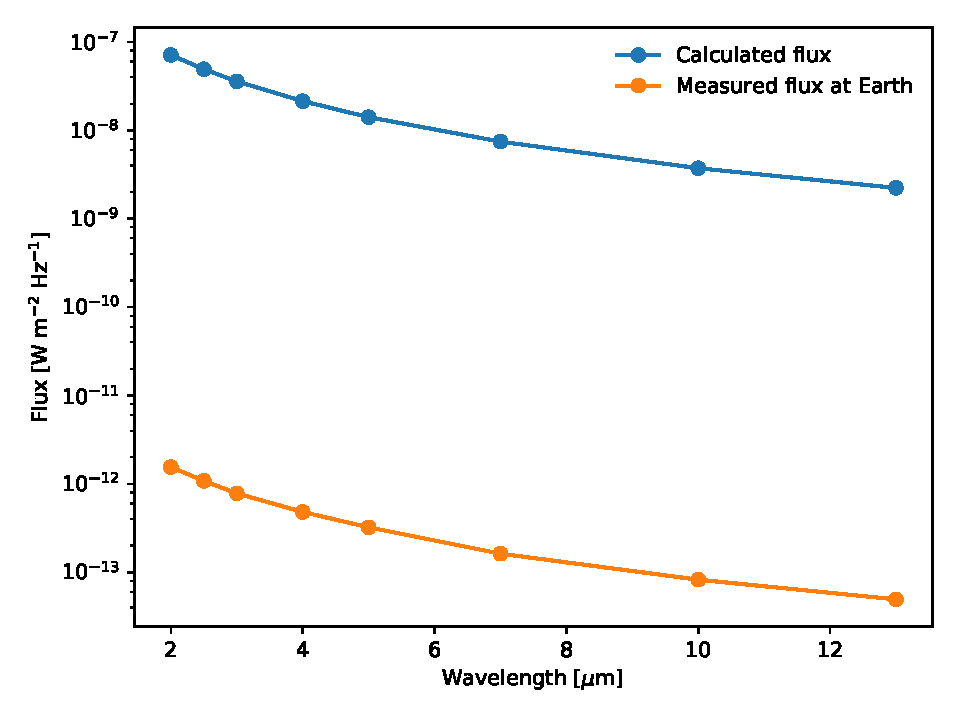
\includegraphics[width=0.85\linewidth]{figures/IRFM.pdf}
    \caption{Measured and calculated flux from the Sun at infrared wavelengths. Data from Table 2 in
             \citet{Blackwell1977}. Mean solar radius from this data is $1.011R_\odot$, and mean
             solar $T_\mathrm{eff}=\SI{5963}{K}$ using \eref{eq:irfm}.}
    \label{fig:IRFM}
\end{figure}

The main drawbacks of the IRFM is the model dependence, a drawback many methods share, and the need
of high precision infrared photometry. For the model atmosphere a metallicity and surface gravity is
assumed which has an effect on $\mathcal{F}_S$, and hence on the final derived $T_\mathrm{eff}$ and
$R$. A more in-depth description of the IRFM can be see in e.g. \citet[][section 4]{Casagrande2006}.


\subsection{$T_\mathrm{eff}$-colour-$[\ion{Fe}/\ion{H}]$ calibration}

Photometry can be used for deriving $T_\mathrm{eff}$ using existing colour calibrations like that of
for example \citet{Ramirez2005a} where adopted $T_\mathrm{eff}$ and $[\ion{Fe}/\ion{H}]$ in
combination with colours such as $B-V$, $V-S$, etc. are used to fit a polynomial such that the
$T_\mathrm{eff}$ can easily be estimated with a simple relation:
\begin{align}
  T_\mathrm{eff} = \frac{5040}{\theta_\mathrm{eff}} + P(X, [\ion{Fe}/\ion{H}]),
\end{align}
where
\begin{align}
  \theta_\mathrm{eff} &= \frac{5040}{T_\mathrm{eff}} \\
                      &= a_0+a_1 X+a_2 X^2+a_3X[\ion{Fe}/\ion{H}] + a_4[\ion{Fe}/\ion{H}] + a_5[\ion{Fe}/\ion{H}]^2
\end{align}
is the polynomial fit between $T_\mathrm{eff}$ versus a colour ($X$) and the metallicity. The
polynomial $P(X, [\ion{Fe}/\ion{H}])$ is a correction applied to remove trends in the residuals, for
example spectral features such as the Balmer lines or the Paschen jump. This correction is performed
after the initial fit.

After obtaining the coefficients ($a_i$) for different combinations of colours, it is trivial to
obtain $T_\mathrm{eff}$ if the metallicity and a colour is known of the star.

\subsection{Asteroseismology}

Asteroseismology is the study of stellar pulsations. These pulsations propagate as sounds waves
throughout a star, their origin and amplitude is determined by the characteristics of the star,
hence the study of the pulsations, which are seen on the surface, will thus be a study of the
stellar properties. In order to to study these a time series is needed. This can both be radial
velocities as it was used in the recent results from the SONG telescope \citep{Grundahl2017}, or
photometry like the numerous results from e.g. the space telescopes \emph{CoRoT} and \emph{Kepler}
\citep[see e.g.][]{Christensen-Dalsgaard2010,Huber2014,Chaplin2011}. The analysis is identical for
either time series, however the amplitudes in the power spectrum will look different.

After determining the frequencies of a range of pulsations from a power spectrum of the time series,
a pattern emerge at every $\Delta\nu$ (the so-called large frequency separation). A finer pattern
also occur described by $\delta\nu$. Last the frequency at maximum power is also measured from the
power spectrum, $\nu_\mathrm{max}$. These frequency separations are used to obtain $\log g$ via
\begin{align}
  \nu_\mathrm{max} &\propto \frac{g}{\sqrt{T_\mathrm{eff}}} \\
                   &= \frac{M/M_\odot}{(R/R_\odot)^2 \sqrt{T_\mathrm{eff}/5777}}\; \SI{3.05}{mHz},\label{eq:scaling1}
\end{align}
where $\nu_{\mathrm{max},\odot}=\SI{3.05}{mHz}$ is the frequency of maximum amplitude for the Sun. A
similar equation exists for the determination of the stellar density:
\begin{align}
  \Delta\nu = (M/M_\odot)^{-1/2} (R/R_\odot)^{-3/2}\; \SI{134.9}{\micro\hertz}.
\end{align}
These simple scaling relation are described in detail in \citet{Kjeldsen1995}. These two equations
can be used together to determine the mass and radius of the star, often to a high precision. These
scaling relations are applicable for stars which shows solar-like oscillations, mostly found in main
sequence FGK stars, but can also be found in red giant stars. The mass and radius for a range of
$\nu_\mathrm{max}$ and $\Delta\nu$ can be seen in \fref{fig:scaling}, where
$T_\mathrm{eff}=\SI{5777}{K}$. The star located at $\{\Delta\nu=\SI{134.9}{\micro
Hz};\;\nu_\mathrm{max}=\SI{3.05}{mHz}\}$ is the Sun.

The small frequency separation, $\delta\nu$, is sensitive to the sound-speed gradient in the core
which in turn is sensitive to the composition. Thus the small frequency separation is a very
important diagnostic for stellar evolution. An interesting case is that of \citet{Bedding2011},
where it was shown it is possible to distinguish between hydrogen- and helium-burning cores in red
giant stars.

\begin{figure}[htpb!]
    \centering
    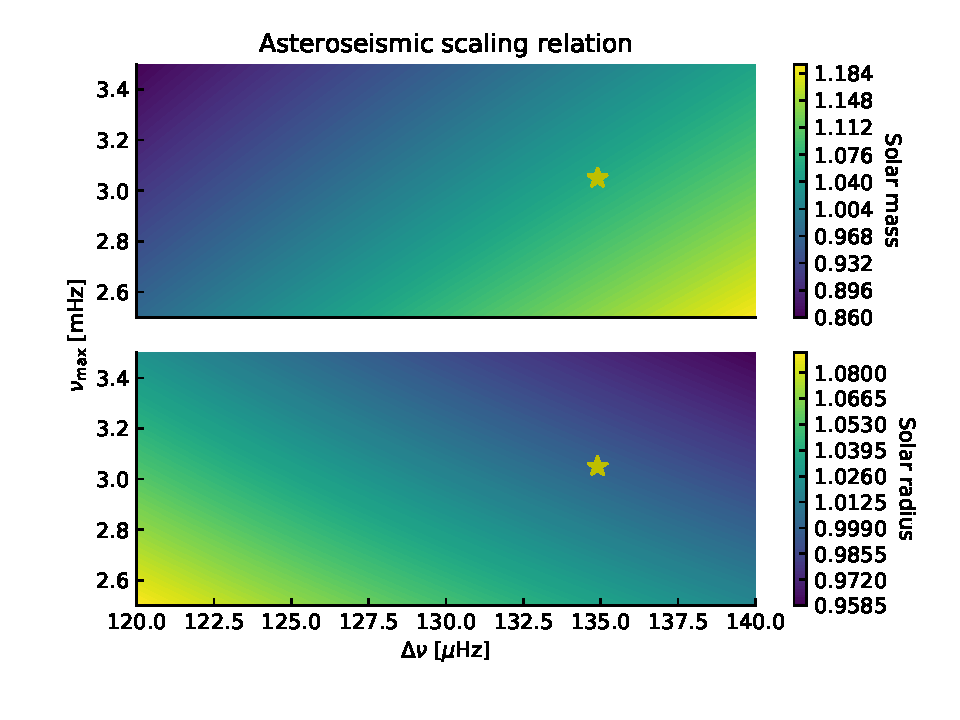
\includegraphics[width=0.85\linewidth]{figures/scaling_relation.pdf}
    \caption{Mass and radius from asteroseismic scaling relation. The colour is the mass and radius
             for the upper and lower panel, respectively.}
    \label{fig:scaling}
\end{figure}

A drawback of asteroseismology is the dependence of $T_\mathrm{eff}$ in \eref{eq:scaling1} which has
to be provided from another method. Ideally this will come from spectroscopy for which the
determination of $T_\mathrm{eff}$ is often reliable. This drawback is minor compared to the lack of
model dependence which is one of the strongest advantages of asteroseismology.

For both of the mentioned photometric methods to determine some atmospheric parameters a
disadvantage is the dependence on the knowledge of other atmospheric parameters which usually comes
from spectroscopy (e.g. metallicity). However, as will be discussed in
\sref{sec:method_spectroscopy} $\log g$ is often difficult to determine reliably and synergies are
welcomed between different methods.

\section{Spectroscopy}
\label{sec:method_spectroscopy}

A spectrum can be analysed with a range of different methods. The method finally chosen depend on
quality of the spectrum, i.e. high/low resolution and high/low S/N, the spectral type of the star,
the region that was observed, e.g. UV, optical, NIR, etc., some stellar properties, e.g.
fast-rotator, activity, etc. No methods work for all cases, but sometime several methods can be used
for on case.

Since this thesis is focused on FGKM stars, and mainly dwarfs, three methods will be described;
synthesis, spectral indices, and the EW method. The latter method will be described in a separate
section since this is the main method used for the analysis in this thesis.



\subsection{Synthesis}
\label{sec:synthesis}

The synthesis fitting method is a standard method for obtaining stellar atmospheric parameters from
a wide range of spectra, that is with different spectral resolution, spectral parameters such as
$T_\mathrm{eff}$, $\log g$, $v\sin i$ the projected rotational velocity, etc., and S/N  \citep[see
e.g.][]{Tsantaki2017}. The synthetic fitting method is in simple terms a comparison between the
observed spectrum and a synthetic spectrum, which is either calculated on the fly like Spectroscopy
Made Easy (SME) \citep{Valenti1996}, or using a pre-calculated grid like Starfish
\citep{Czekala2015}. By analysing the
\begin{align}
  \chi^2 = \sum_i^N\frac{(y_\mathrm{obs,i}-y_\mathrm{model,i})^2}{\sigma_i},
\end{align}
the synthetic spectrum that best match the observed spectrum can be found. Here the $y_\mathrm{obs}$
is the observed spectrum, $y_\mathrm{model}$ is the synthetic spectrum, and $\sigma$ is the error on
the measurement.

The synthetic fitting can be done by utilising small windows around sensitive spectral features such
as ionized lines or hydrogen lines for obtaining the surface gravity, iron lines for obtaining the
effective temperature, a series of different atomic lines for obtaining the overall metallicity.
This approach is used by FASMA and SME \citep[][respectively]{Valenti1996,Tsantaki2017} and is a
compromise between fitting the entire spectral range and calculating the synthetic spectra on the
fly which is time consuming. On the other hand the entire spectrum can be fitted if a pre-calculated
grid of synthetic spectra are available. By masking small windows, one can also exclude different
features that are troublesome, this can be telluric lines, bad reduction of the spectra, or real
spectral features where there currently is poor atomic/molecular data such as the oscillator
strength and thus it is not possible to reliably fit this feature.

This method is affected by the different approaches one can use, that is which atmosphere models are
used (ATLAS, MARCS, etc.), atomic data and whether this has been calibrated, the radiative transfer
code in the case the synthetic spectra are calculated on the fly, and the minimization procedure
chosen. With these things in mind it is important to stress the wide range spectra and spectral
classes this method works with.




\section{\code{FASMA}}
\label{sec:parameters}

The EW method or curve-of-growth analysis is another standard method for obtaining stellar
atmospheric parameters from spectra as the synthetic fitting method (\sref{sec:synthesis}). Since
this is the method used throughout this thesis it will be explained in detail. This analysis follow
a chain of tasks, each has been made automatic in the software Fast Analysis of Spectra Made
Automatically (\code{FASMA}\footnote{Greek for spectrum}) which was developed during this thesis
\citep{Andreasen2017a}. \code{FASMA} is made of three \code{drivers}:
\begin{enumerate}
  \item EW measurement driver
  \item Obtain stellar atmospheric parameters driver
  \item Abundance driver
\end{enumerate}
An additional driver is under development; a synthetic fitting driver \citep{Tsantaki2017}.
\code{FASMA} has been made available to the community via a web application at
\url{http://www.iastro.pt/fasma/}.


\subsection{Ingredients}

\code{FASMA} is written in the Python programming language and glue together other software and
model atmospheres necessary for obtaining stellar atmospheric parameters from high quality spectra.
These software and models are described in greater detail in the following sections. In short, the
curve-of-growth analysis require measured EWs where the latest version\footnote{The latest version
can be found here: \url{https://github.com/sousasag/ARES}} of \code{ARES} is used
\citep{Sousa2015a}. These EWs are used to derive line abundances using model atmosphere like the
ATLAS9 \citep{Kurucz1993}, MARCS models \citep{Gustafson2008}, or PHOENIX models \citep{Husser2013}
to mention the most popular for this analysis. Note that the PHOENIX models are relative new and not
as widely used yet. In tandem with model atmospheres a radiative transfer code is also needed.
\code{FASMA} uses \MOOG \citep{Sneden1973} for this. The model atmosphere usually comes in a
pre-calculated grid in the $\{T_\mathrm{eff},\,\log g,\,[\ion{Fe}/\ion{H}]\}$ parameter space. These
are interpolated in order to access the requested combination of parameters. Last, \code{FASMA}
consist of a minimization routine which looks for the best matching parameters given a spectrum.



\subsection{Wrapper for \code{ARES}}
\label{sec:measureEW}

There are two ways to measure the EW of an absorption line, manually or automatically. There are
advantages and disadvantages for both method. For the manual, an advantage is that we can inspect
the lines and try to measure lines in different ways (which is useful if it is blended). We have
more control over how blended lines are fitted, and which profiles are used. Disadvantages are that
it is very time consuming, and it is prone to errors, as a measurement might change drastically by
the eyes measuring it. Even for the same person, the measurement can change. By mentioning the
advantages and disadvantages of the manual method, it should be clear that the advantages and
disadvantages of the automatic method is the opposite of those. Especially the time to measure the
lines are orders of magnitudes faster, which is crucial when dealing with more than a handful of
spectra.

When a line is measurement by hand (manually) it is in this thesis done using the \code{splot}
command in \code{IRAF}. Here the deblending mode is used whenever necessary. It is often necessary
to fit one spectral lines with several Gaussians, as neighbouring lines might contaminate the line
of interest.

When a line is measurement automatically it is in this thesis done with \code{ARES}
\citep{Sousa2007,Sousa2015a}. When using \code{ARES} it is important to use a correct value of the
\code{rejt} parameter. This parameter is used for placing the continuum level, and is thus directly
related to the final measurement EW. It is difficult to get this parameter right, however the newest
version of \code{ARES} has the option to analyse a few absorption free regions and measure the S/N.
The \code{rejt} is then calculated as:
\begin{align*}
  \mathtt{rejt} = 1 - \frac{1}{\mathrm{S/N}}.
\end{align*}

\code{ARES} is used via the first driver of \code{FASMA}. All the options available for \code{ARES}
can be accessed by \code{FASMA}. The options are
\begin{itemize}
  \item Setting the spectral window, $\lambda_\mathrm{min}$ and $\lambda_\mathrm{max}$
  \item RV correction to be applied or a mask to measure the RV and automatic make this correction
  \item minimum and maximum EW to be considered ($\SI{5}{m\angstrom}$ and $\SI{150}{m\angstrom}$
        respectively by default)
  \item Minimum distance between two consecutive lines
  \item Smoothing applied with a \code{boxcar} filter before measuring the EWs
\end{itemize}
An in-depth description of these options can be found in
\citet{Sousa2007,Sousa2015a}.

Sometimes \code{ARES} crash when measuring an absorption line. The reason is not clear, however when
dealing with a large amount of spectra, it is important that the analysis moves on. To deal with
this problem, \code{FASMA} finds the last line which \code{ARES} tried to measure in the log file. This line is
temporarily removed from the line list and \code{ARES} is restarted. The line list used for deriving
parameters consists of numerous iron lines, thus removing one line will have a negligible effect on
the final derived parameters.



\subsection{Interpolation of atmosphere models}
\label{sec:interpolation}

\code{FASMA} has access to both ATLAS9 models by \citet{Kurucz1993} and MARCS models by
\citet{Gustafson2008}, both are in a pre-calculated grid as described above. Let this grid be
described by $\{T_\mathrm{eff,g},\, \log g_g,\, [\ion{Fe}/\ion{H}]_g\}$, where subscript $g$ is one
of the grid points. Such a grid can be seen in \fref{fig:grid} for $[\ion{Fe}/\ion{H}]=0.00$ in the
$T_\mathrm{eff}$ range; $\SIrange{3000}{10000}{K}$. For visualisation the location of the Sun is
shown as well. The colour scale corresponds to the temperature in the first layer of each model
atmosphere, i.e. the uppermost layer. The requested value will be $\{T_\mathrm{eff,r},\,\log
g_r,\,[\ion{Fe}/\ion{H}]_r\}$. The task is now to find the surrounding grid points in the parameter
space of the requested parameters. For $\log g$ and $[\ion{Fe}/\ion{H}]$ two neighbouring grid point
are used, and for $T_\mathrm{eff}$ four surrounding grid point are used, in total
$4\times2\times2=16$ model atmospheres for the interpolation. \code{FASMA} use the four surrounding
grid points for $T_\mathrm{eff}$ instead of two, since the model atmosphere changes most with
$T_\mathrm{eff}$. This is common in other interpolations as well \citep[see e.g.][]{Valenti1996}.

\begin{figure}[htpb!]
    \centering
    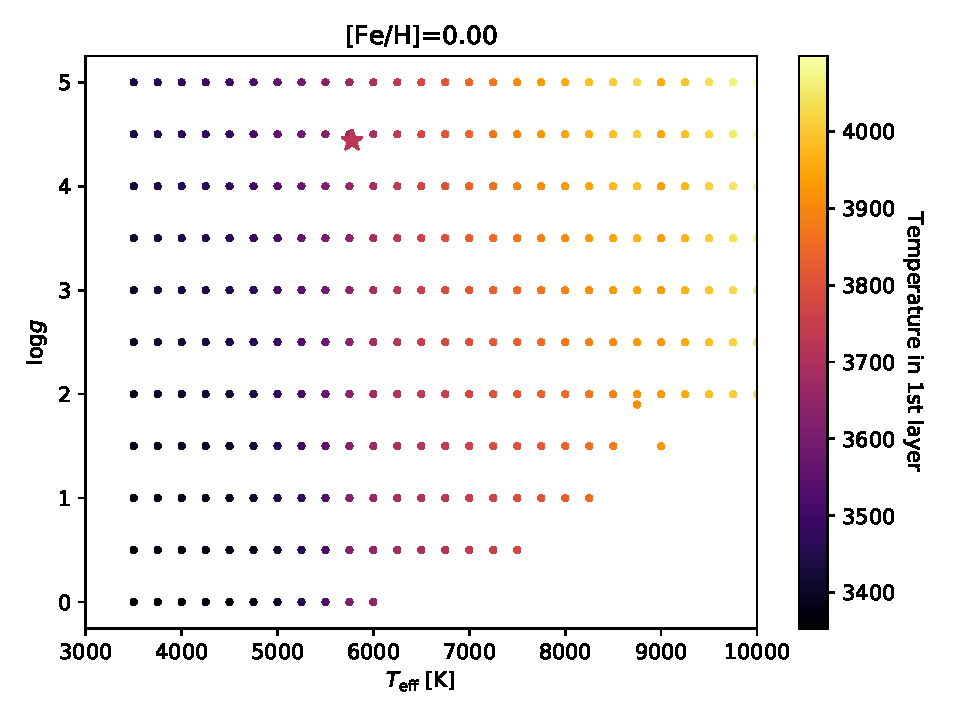
\includegraphics[width=0.85\linewidth]{figures/model_atmosphere.pdf}
    \caption{Model atmosphere grid from \citet{Kurucz1993} at $[\ion{Fe}/\ion{H}]=0.00$ between
             \SI{3000}{K} and \SI{10000}{K}. The grid extends to higher $T_\mathrm{eff}$, but these
             are not considered in this thesis.}
    \label{fig:grid}
\end{figure}

When the 16 model atmosphere have been located, the interpolation goes through each layer of the
model atmosphere, where there typical are 72 layers, and each column of which there are six. The
columns are described in \sref{sec:atmospheremodels}. The interpolation are done using the
\code{griddata} function from \code{SciPy}\footnote{\url{https://scipy.org/}}. The interpolation is
linear in the parameter space. After the interpolation, the result is saved to a file in the format
expected by \MOOG.




\subsection{Minimization}

With the measured EWs for all the lines in the line list, we choose an atmosphere model to determine
the abundances. If there is no prior knowledge of the star it is common simply to choose an
atmosphere model with solar parameters as a starting point. Once the line abundances of all the iron
lines has been determined, the linear correlation between the abundances and the reduced EWs (RW),
and the abundances and the excitation potential is calculated. If there is a correlation it means
the model atmosphere used is wrong. Moreover, we also have to check if the mean abundance of
\ion{Fe}{I} and \ion{Fe}{II} lines are equal, and last if mean abundance of the \ion{Fe}{I} lines is
equal to the input $[\ion{M}/\ion{H}]$ of the atmosphere model\footnote{We use \ion{Fe}{I} instead
of \ion{Fe}{II} lines for this, since they are more numerous.}. If one of these four criteria does
not pass, then the atmosphere model is wrong, and we have to search for a new one. A common way to
do this, is by combining the indicators into a scalar value:
\begin{align}
  f(\{T_\mathrm{eff}, \log g, [Fe/H], \xi_\mathrm{micro}\}) &= \sqrt{a_\mathrm{EP}^2 + a_\mathrm{RW}^2 + \Delta\ion{Fe}{}^2},
\end{align}
where $a_\mathrm{EP}$ is the correlation between abundances and excitation potential,
$a_\mathrm{RW}$ is the correlation between abundances and RW, and $\Delta\ion{Fe}{}$ is the
difference between the mean abundances of \ion{Fe}{I} and \ion{Fe}{II}. This scalar function can be
minimized using standard minimization procedures as the simplex downhill among others. However,
there is another approach that takes into the account the information stored in these indicators.
For example, if $a_\mathrm{EP}$ is positive it means $T_\mathrm{eff}$ has to be increased by an
amount correlated by the numerical value of $a_\mathrm{EP}$. In the same way, a non-zero
$a_\mathrm{RW}$ means $\xi_\mathrm{micro}$ has to be changed, and $\Delta\ion{Fe}{}$ is an indicator
for $\log g$. In the end it is a vector function being minimized which are more difficult, however
we are not minimizing this using standard mathematical methods, but rather using the physical
knowledge. This minimization is useless for anything else, but it is excellent for this. The vector
function has the form:
\begin{align}
    f(\{T_\mathrm{eff}, \log g, [Fe/H], \xi_\mathrm{micro}\}) = \{a_\mathrm{EP}, a_\mathrm{RW}, \Delta\ion{Fe}, \ion{Fe}{I}\}.
\end{align}

The abundances of \ion{Fe}{I} lines versus EP and RW are shown in \fref{fig:eprw} for the planet
host star HATS-1. The three rows are for three different model atmospheres. From upper to lower:
\begin{itemize}
  \item Converged: $T_\mathrm{eff}=\SI{5959}{K}$,
                   $\log g=4.59$,
                   $[\ion{Fe}/\ion{H}]=-0.04$, and
                   $\xi_\mathrm{micro}=\SI{1.05}{km/s}$.
  \item Converged with \SI{0.5}{km/s} added to $\xi_\mathrm{micro}$.
  \item Converged with \SI{500}{K} added to $T_\mathrm{eff}$.
\end{itemize}
Left column show the abundances against the EP, and the right column is
abundances against RW.

\begin{figure}[htpb!]
    \centering
    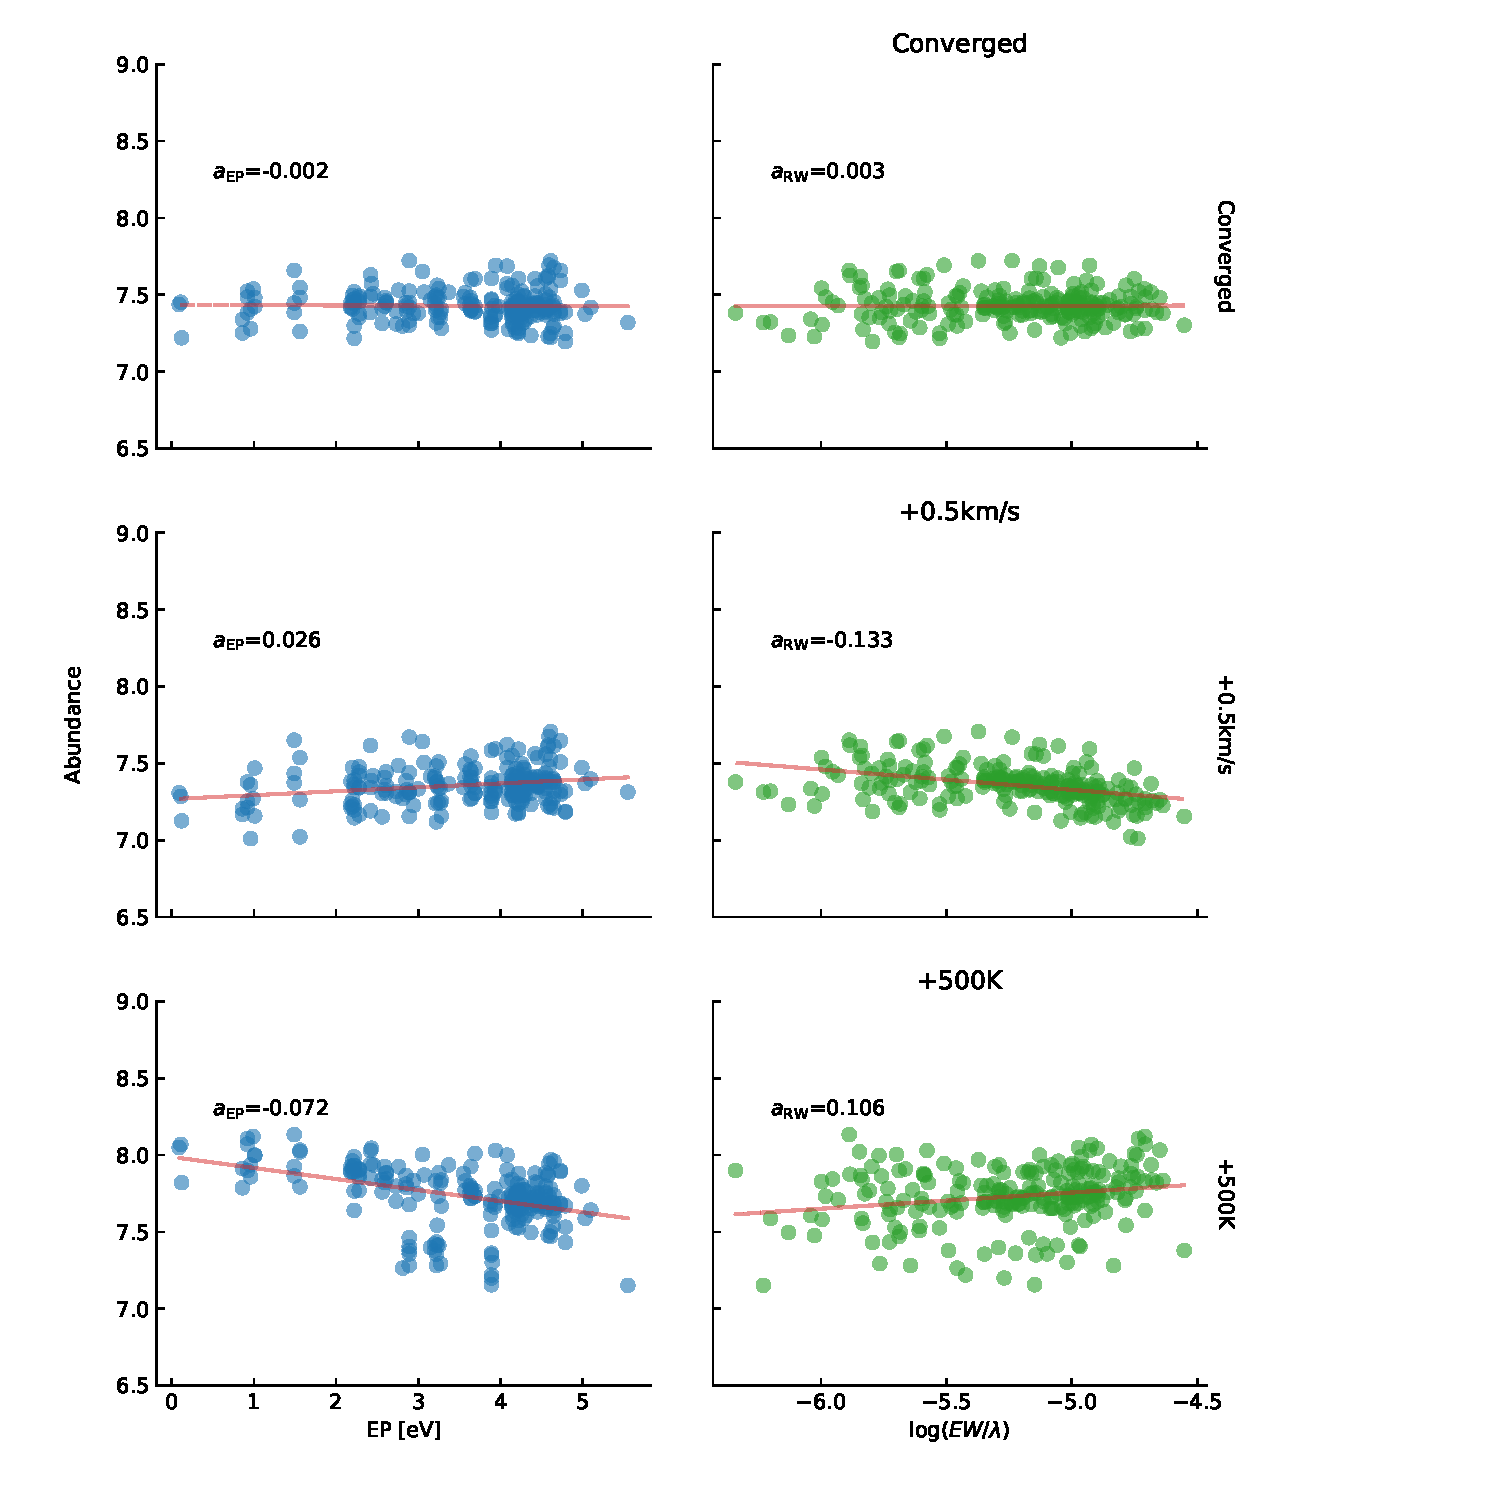
\includegraphics[width=0.85\linewidth]{figures/EP_RW_vs_abundance.pdf}
    \caption{The abundances of \ion{Fe}{I} for the planet host star: HATS-1.
             Upper plot: Converged parameters (see text for stellar parameters for this star).
             Middle plot: Converged parameters with \SI{0.5}{km/s} added to $\xi_\mathrm{micro}$.
             Lower plot: Converged parameters with \SI{500}{K} added to $T_\mathrm{eff}$.}
    \label{fig:eprw}
\end{figure}

The minimization with the different options is depicted in \fref{fig:minimization}. In each
iteration where convergence is not reached, the input metallicity is changed to that of the average
output metallicity using the \ion{Fe}{I} lines. \code{FASMA} is able to fix one or all of the four
atmospheric parameters, and when it reach convergence it checks if there are any outliers in the
abundances. These will be removed, either:
\begin{itemize}
  \item All outliers above $3\sigma$ once; minimization routine is restarted after removal of
        outliers.
  \item All outliers above $3\sigma$ iteratively; minimization routine is restarted after removal of
        outliers each time.
  \item One outlier above $3\sigma$ (with the highest deviation) is removed iteratively;
        minimization routine is restarted after removal of outliers each time.
\end{itemize}

All restarts of the minimization will start at the precious best found parameters. For the latter
two were outliers are removed iteratively, this will continue until no outliers are present. An
optical line list like the ones by \citet{Sousa2008a,Tsantaki2013} have been tested thoroughly and
it is safe to remove a larger amount of lines and still obtain reliable parameters, thus using the
first option is common here. However, with a less tested line list, like the one by
\citet{Andreasen2016} (and refined in \citet{Andreasen2017b}), one should remove outliers more
carefully, and it is recommended that one outlier is removed iteratively.

Sometimes the minimization can not reach convergence with all parameters free. The first approach to
progress is to fix $\xi_\mathrm{micro}$ to a value. This parameter is known to depend on the
spectral type \citep[see e.g.][and references therein]{Tsantaki2013}. \code{FASMA} use one of two
empirical relations to fix $\xi_\mathrm{micro}$ if this is close to either $0\si{km/s}$ or
$5\si{km/s}$ and $|a_\mathrm{RW}| > 0.050$ at the end of the minimization. The empirical relations
are:
\begin{align}
  vt =
  \begin{cases}
    6.935 \cdot 10^{-4}\; T_\mathrm{teff} - 0.348 \log g - 1.437     & \text{For $\log g \ge 3.95$} \\
    2.72 - 0.457 \log g + 0.072 \cdot [\ion{Fe}/\ion{H}]             & \text{For $\log g < 3.95$},
  \end{cases}
\end{align}
where the first case is from \citet{Tsantaki2013} and the latter case is from \citet{Adibekyan2015}.
In this way $\xi_\mathrm{micro}$ is changed in each iteration according to one of these relations.
This option is called \code{autofixvt} in \fref{fig:minimization}.

Last there is an option, \code{refine}. This apply more strict criteria for the indicators to reach
convergence, thus making the minimization less sensitive to the initial guess since it could
otherwise reach convergence from one "side" of the parameter space. The default criteria are:
\begin{align*}
  a_\mathrm{EP}     &= 0.001\\
  a_\mathrm{RW}     &= 0.003\\
  \Delta\mathrm{Fe} &= 0.001.
\end{align*}
The criteria for $a_\mathrm{RW}$ is not as strict as $a_\mathrm{EP}$ since this indicator can change
rapidly with small changes in $\xi_\mathrm{micro}$, thus a very strict criteria might never lead to
convergence. Convergence is reached once all of the above criteria are met, and the input and output
metallicity are identical. If one or more of the parameters are fixed, the corresponding criterion
is simply set to 0 and effectively ignored, thus not changing the parameter.

For each iteration, the change to be applied for the atmospheric parameters are defined by adding
the following:
\begin{align}
  T_\mathrm{eff}     &: \SI{2000}{K} \cdot a_\mathrm{EP}   \\
  \xi_\mathrm{micro} &: \SI{1.5}{km/s} \cdot a_\mathrm{RW} \\
  \log g             &: -\Delta\mathrm{Fe}
\end{align}
to each parameter. Note again that metallicity is simply changed to the the output metallicity of
the previous iteration. These are empirical relations. Note that by changing e.g. $T_\mathrm{eff}$
not only is $a_\mathrm{EP}$ affected, but the other indicators as well as seen in \fref{fig:eprw}.
This inter-dependency between the parameters is ignored by \code{FASMA} as it is not a simple
problem to solve. The stepping presented above is chosen to rapidly reach convergence, without
causing problems for the inter-dependency.

\begin{figure}[htpb!]
    \centering
    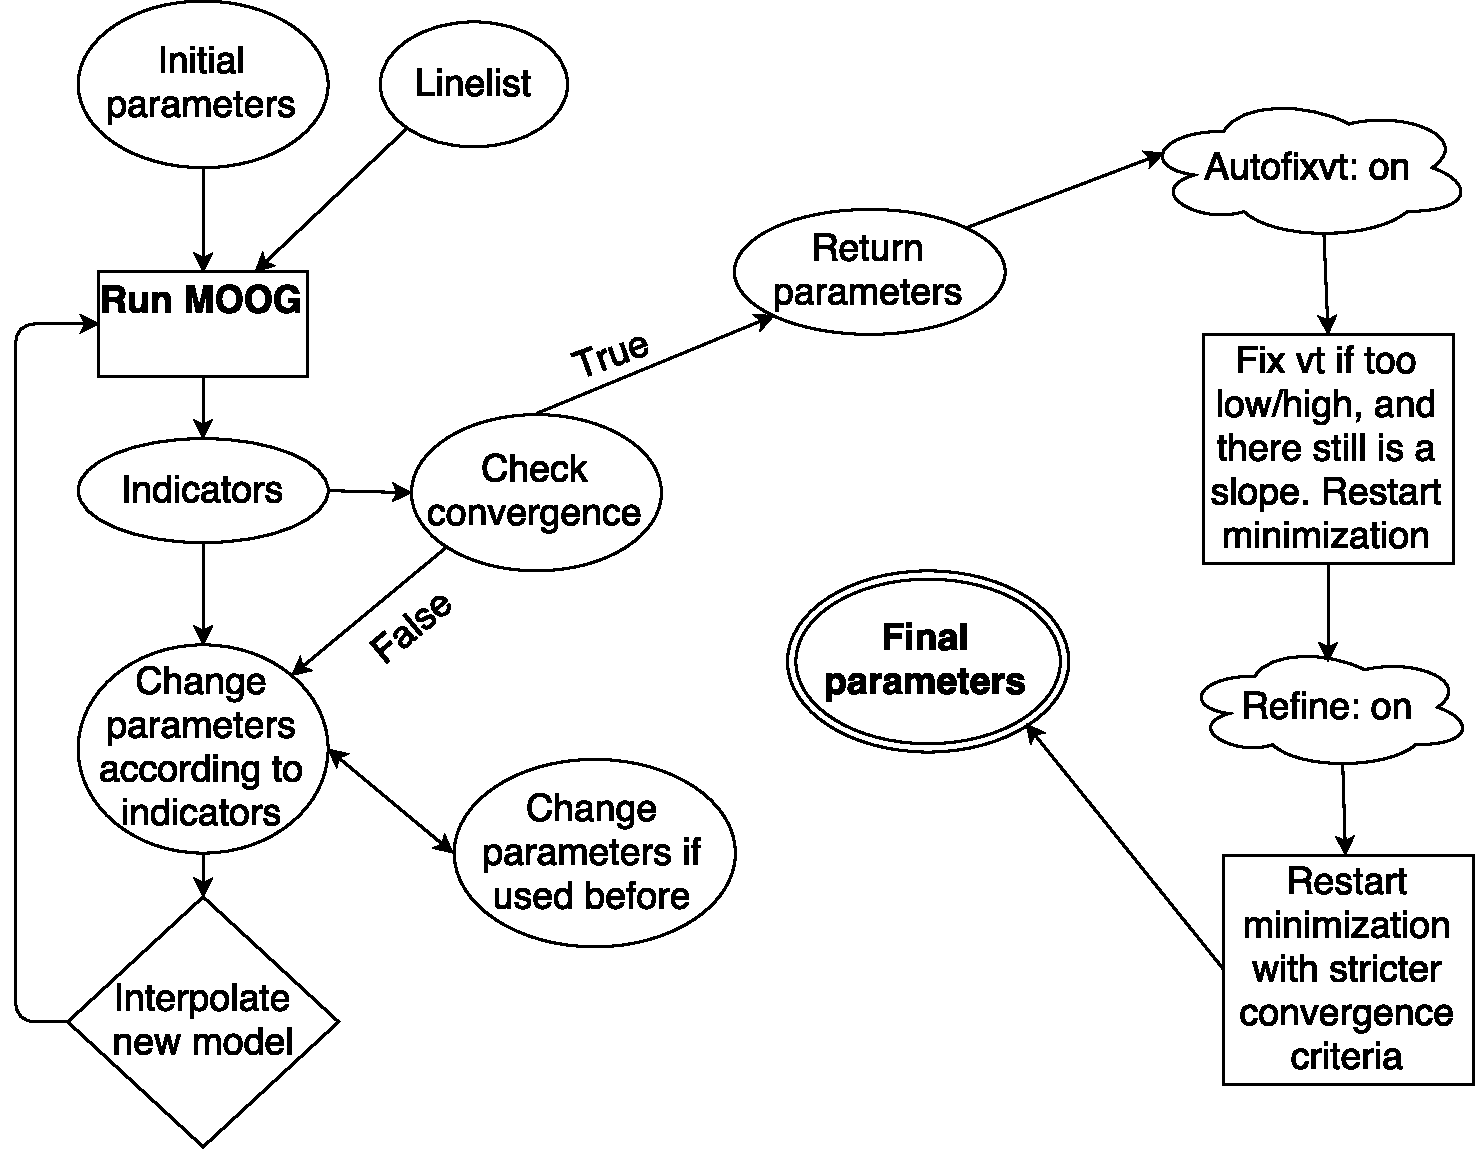
\includegraphics[width=0.85\linewidth]{figures/FASMA_minimization.pdf}
    \caption{Overview of the minimization for \code{FASMA}. Credit: \citet{Andreasen2017a}.}
    \label{fig:minimization}
\end{figure}


\subsection{Error estimate}
\label{sec:error_estimate}

The error estimate is based on the same method presented in \citet{Neuforge1997}. The error on
$\xi_\mathrm{micro}$ corresponds to the $1\sigma$ statistical error on the slope of the linear
regression between \ion{Fe}{I} abundances and RW. The error on $T_\mathrm{eff}$ is the statistical
error on the slope between \ion{Fe}{I} abundances and EP as well as the uncertainty in
$\xi_\mathrm{micro}$. The error for $[\ion{Fe}/\ion{H}]$ corresponds to the dispersion of the
\ion{Fe}{I} abundances as well as the uncertainties in $\xi_\mathrm{micro}$ and $T_\mathrm{eff}$.
The error in $\log g$ corresponds to the dispersion in the pressure sensitive \ion{Fe}{II}
abundances.
